\section{Bayesian Updating}
\label{sec:02_filter}

Assuming gaussian distribution of the single robot results,
the multi-agent decision process is done by Bayesian Updating.
One dimensional probability density functions of states with
variance $\sigma^2$ and mean $\mu$ are described as
\bal
    \mathcal{N}(x,\sigma,\mu) = \frac{1}{\sigma\sqrt{2\pi}}e^{-\frac{(x-\sigma)^2}{2\sigma^2}}.
    \label{eq:02_probabilityDensity}
\eal
Having two values $\mu_0$ and $\mu_1$ with their variances,
the result $\mu'$ of the combination of both is
\bal
    \mathcal{N}(x,\sigma',\mu') = \mathcal{N}(x,\sigma_0',\mu_0') \cdot \mathcal{N}(x,\sigma_1',\mu_1').
    \label{eq:02_newProbabilityDensity}
\eal
By substitution and conversion, $\mu'$ and $\sigma'^2$ can be
formulated to
\bsub
\label{eq:02_intersectionState}
\bal
    \mu' &= \mu_0 + \frac{\sigma_0^2(\mu_1-\mu_0)}{\sigma_0^2+\sigma_1^2}\\
    \sigma'^2 &= \sigma_0^2 - \frac{\sigma_0^4}{\sigma_0^2+\sigma_1^2}.
\eal
\esub

\subsection{Two Dimensional Case}
\label{subsec:02_2dTeam}

Imaging having results from two agents that accomplished the \ac{WSDE} algorithm by
computing the \ac{TDOA} with any method, either the \ac{WSDE} angles of both robots
cross and an intersection point would be found or no final whistle source position result arises.
Each of these intersection points can be interpreted as whistle source positions
with given state $\mu$ and variance $\sigma$ of \cref{eq:02_probabilityDensity}.
Final whistle source position of all robots is estimated by iterating over
all intersections and updating the result with \cref{eq:02_intersectionState}.

Exemplary, two robots at position $\vec{p_j}$ and $\vec{p_k}$ with their \ac{WSDE} results
are illustrated in \cref{fig:03_rays}.
\begin{figure}[ht]
	\centering
		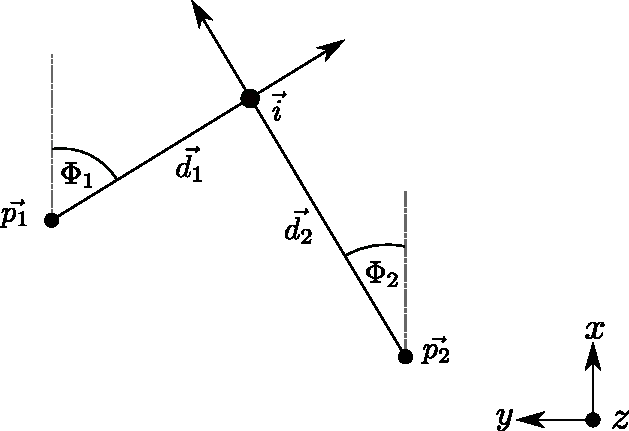
\includegraphics[width=0.50\textwidth]{figures/rays}
    \caption[Nomenclature for multi-agent localization algorithm]
            {Nomenclature for multi-agent localization algorithm.}
    \label{fig:03_rays}
\end{figure}
% -------------------------------------------------------------

Every \ac{WSDE} result is represented as \textit{ray} which consists of the robot position
$\vec{p_j}$ and the \ac{WSDE} angle $\Phi_j$, both in field coordinates.
The \ac{WSDE} angle $\gamma_j$ is defined relative to the robot and the robot's orientation $\theta_j$
is known by its team message information.
Thus, the absolute angle is
\bal
\Phi_j &= \theta_j + \gamma_j\\
\intertext{from which the whistle source direction ray can be described as}
\vec{r_j} &= \vec{p_j} + \vec{d_j} % = \begin{pmatrix}p_{jx}\\p_{jy}\end{pmatrix} + \ell \begin{pmatrix}d_{jx}\\d_{jy}\end{pmatrix}
    = \begin{pmatrix}p_{jx}\\p_{jy}\end{pmatrix} + \ell \begin{pmatrix}\cos(\Phi_j)\\\sin(\Phi_j)\end{pmatrix}.
\label{eq:03_ray}
\eal

An intersection point of two rays $\vec{r_j}$ and $\vec{r_k}$ is expressed as
\bal
    \vec{i_{jk}} &= \begin{pmatrix}i_{jkx}\\i_{jky}\end{pmatrix}
\eal
with x- and y-coordinates.
If two real numbers $u$ and $v$ exist, so that
\bal
    \vec{i_{12}} &= \vec{p_1} + u \cdot \vec{d_1} = \vec{p_2} + v \cdot \vec{d_2}
    \label{eq:03_intersection}
    \\
    \intertext{a intersection point can be determined by simple geometrical relations.
               With the given terms and conditions $u$ and $v$ values are computed by
               dividing the vectors into x- and y-value and solving the equations, resulting in}
    u &= \frac{p_{1y} \cdot d_{2x} + d_{2y} \cdot p_{2x} - p_{2y} \cdot d_{2x} - d_{2y} \cdot p_{1x}}
            {d_{1x} \cdot d_{2y} - d_{1y} \cdot d_{2x}}
            \label{eq:03_intersectionU}
            \\
    v &= \frac{p_{1x} + d_{1x} \cdot u - p_{2x}}{d_{2x}}.
\eal
% -------------------------------------------------------------

% DEFINITION COVARIANCE MATRIX
The covariance matrix $\textbit{C}_{jk}$ is obtained in the spirit of an Extended Kalman filter \cite{kalman}
considering the Jacobian matrix $\textbit{J}_{jk}(\Phi_j, \Phi_k)$ and the average angle error $\varepsilon_{\Phi}$
over all available measurements.
Expressing the direction vector $\vec{d}_j$ of the ray by angle $\Phi_j$ as in \cref{eq:03_ray}, the covariance
matrix of the intersection of two rays $\vec{r}_j$ and $\vec{r}_k$ is
\bsub
\label{eq:03_cov}
\bal
\textbit{C}_{jk} &= \left( \begin{matrix}
                        \varepsilon_{\Phi} & 0 \\
                        0 & \varepsilon_{\Phi} \\
                      \end{matrix} \right) \cdot \textbit{J}_i(\Phi_j, \Phi_k)
\\
\intertext{with the Jacobian matrix}
\textbit{J}_i(\Phi_j, \Phi_k) &= \left(\begin{matrix}
    \frac{\partial ix}{\partial \Phi_j} & \frac{\partial ix}{\partial \Phi_k} \\
    \frac{\partial iy}{\partial \Phi_j} & \frac{\partial iy}{\partial \Phi_k} \\
    \end{matrix}\right).
\eal
\esub
The elements of the Jacobian result by derivation of the intersection formula \cref{eq:03_intersection}
with \cref{eq:03_intersectionU,eq:03_ray} and yield
\begin{align*}
\frac{\partial ix}{\partial \Phi_1} &= \frac{(\cos(\Phi_2) \cdot (\cos(\Phi_1)^2 + \sin(\Phi_1)^2) \cdot ((p_{1y} - p_{2y}) \cdot \cos(\Phi_2) +
                                  (-p_{1x} + p_{2x}) \cdot \sin(\Phi_2)))}
                                  {(-\cos(\Phi_2) \cdot \sin(\Phi_1) + \cos(\Phi_1) \cdot \sin(\Phi_2))^2}
                                  \\
\frac{\partial ix}{\partial \Phi_2} &= \frac{-(\cos(\Phi_1) \cdot (\cos(\Phi_2)^2 + \sin(\Phi_2)^2) \cdot ((p_{1y} - p_{2y}) \cdot \cos(\Phi_1) + (-p_{1x} + p_{2x}) \cdot \sin(\Phi_1)))}
                                {(\cos(\Phi_1) \cdot \sin(\Phi_2) - \cos(\Phi_2) \cdot \sin(\Phi_1))^2}
                                \\
\frac{\partial iy}{\partial \Phi_1} &= \frac{(\cos(\Phi_1)^2 + \sin(\Phi_1)^2) \cdot \sin(\Phi_2) \cdot ((p_{1y} - p_{2y}) \cdot \cos(\Phi_2) + (-p_{1x} + p_{2x}) \cdot \sin(\Phi_2))}
                                {(-\cos(\Phi_2) \cdot \sin(\Phi_1) + \cos(\Phi_1) \cdot \sin(\Phi_2))^2}
                                \\
\frac{\partial iy}{\partial \Phi_2} &= \frac{(\cos(\Phi_2)^2 + \sin(\Phi_2)^2) \cdot \sin(\Phi_1) \cdot ((-p_{1y} + p_{2y}) \cdot \cos(\Phi_1) + (p_{1x} - p_{2x}) \cdot \sin(\Phi_1))}
                                {(\cos(\Phi_1) \cdot \sin(\Phi_2) - \cos(\Phi_2) \cdot \sin(\Phi_1))^2}.
%  \label{eq:03_jacobianElements}
\end{align*}
